\documentclass[10pt,letterpaper]{article}
\usepackage[T1]{fontenc}
\usepackage{times,microtype,graphicx,booktabs,float}
\usepackage[font=small,labelfont=bf,labelsep=period,skip=4pt]{caption}
\setlength{\textwidth}{6in}
\setlength{\textheight}{9in}
\setlength{\oddsidemargin}{0.25in}
\setlength{\evensidemargin}{0.25in}
\setlength{\topmargin}{-0.35in}
\setlength{\headheight}{0.15in}
\setlength{\headsep}{0.2in}
\setlength{\parindent}{0pt}
\setlength{\parskip}{4pt}
\setlength{\intextsep}{4pt}
\setlength{\textfloatsep}{9pt}
\newcommand{\reporttitle}[2]{\noindent\rule{\linewidth}{4pt}\par
{\LARGE\bfseries #1\par}\vspace{2pt}\noindent\rule{\linewidth}{1pt}\par
#2\par October 16, 2026\par\vspace{4pt}}
\makeatletter
\renewcommand\section{\@startsection{section}{1}{\z@}{9pt}{4pt}{\large\bfseries}}
\makeatother
\renewenvironment{abstract}{\small\textbf{Abstract}\par}{\par\vspace{3pt}}
\let\originalitemize\itemize
\renewcommand{\itemize}{\originalitemize\setlength{\itemsep}{1pt}\setlength{\parskip}{0pt}\setlength{\parsep}{0pt}}
\let\originalenumerate\enumerate
\renewcommand{\enumerate}{\originalenumerate\setlength{\itemsep}{1pt}\setlength{\parskip}{0pt}\setlength{\parsep}{0pt}}
\begin{document}
\reporttitle{Plant preprocessing benchmark evidence}{Arabidopsis DAP-seq and bulk ATAC; matched-stage comparisons}
\begin{abstract}We reconcile 64 completed method/repetition cases across 6 public-data subsets. In a separate MACS3 test, all 24 CPU-specific comparisons preserved the evaluated peak outputs, with 1-CPU speedups of 4.20 to 6.32 times. Most package alternatives lack evidence of a consistent biological improvement, and the broader species panel remains incomplete. We would retain scientific defaults while evaluating the pinned optimized caller within its tested scope.\end{abstract}
\section*{Setup}
\textbf{Data.} Two SE DAP treatments, four PE DAP treatments and two biological ATAC replicates were sampled at 1-million and 5-million template caps. DAP treatments are not extra biological replicates; repeated execution is not a new experiment.

\textbf{Scoring.} Peak Jaccard is intersecting divided by union peak bases. Held-out FRiP is the fraction of retained fragments overlapping the other biological replicate's peaks. Fixed-region Spearman measures count agreement, not truth. Independent PBM motif support uses matched windows; cost is secondary to these scientific comparisons.

\begin{table}[H]\centering\small\caption{Completed method/repetition cases, not biological sample counts.}
\begin{tabular}{lp{3.4in}r}\toprule
Data & Treatment / replicate identity & Cases \\ \midrule
SE DAP & FUS3, ABI5; assigned control & 16 \\
PE DAP & Four protocol-optimization treatments & 16 \\
Bulk ATAC & SRR4000468 and SRR4000469 & 32 \\
\bottomrule\end{tabular}\end{table}
\section{Depth changes discovery more than these small package differences}
For the 2 ATAC biological replicates, peak Jaccard increases from 0.2404 at 1 million pairs to 0.4858 at 5 million pairs. Held-out FRiP rises from 0.1433 to 0.4601 and from 0.1633 to 0.4023, while peak coverage also increases.

\begin{figure}[H]\centering\makebox[\linewidth][c]{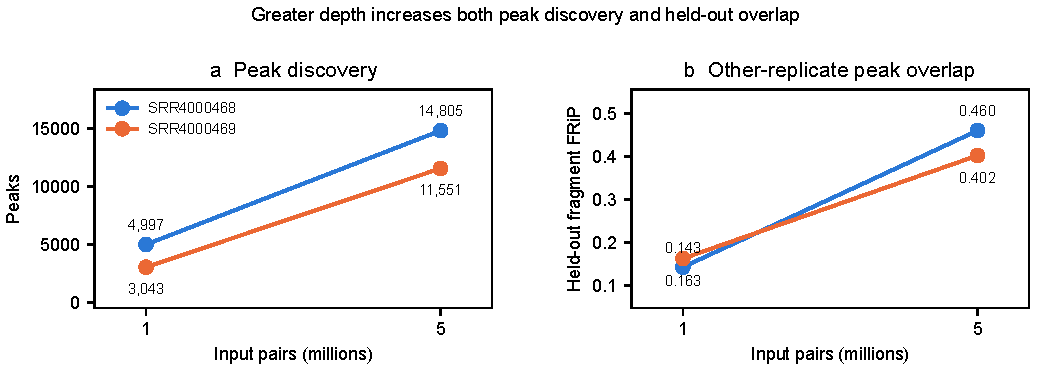
\includegraphics[width=7in]{figures/depth.pdf}}
\caption{TAIR10 baseline peak discovery and cross-replicate overlap.}\end{figure}
\newpage
\section{The current evidence supports scoped decisions}
The 64 cases reconcile to the historical matrix count, but do not represent 64 independent biological experiments. A separate local audit found 8 completed frozen reference baselines and 3 completed assessments; these are not added to the method-matrix denominator.

\begin{table}[H]\centering\small\caption{Decisions supported by the reports in this series.}
\begin{tabular}{p{.85in}p{3.1in}p{1.45in}}\toprule
Step & Observed evidence & Decision \\ \midrule
Alignment & BWA is close; Bowtie2 changes PE DAP peaks & Retain BWA-MEM2 \\
Trimming & Two short-read ATAC replicates change little & Defer general change \\
Duplicates & Picard is faster in one ATAC cohort & Broaden validation \\
Peaks & 24 exact-output optimized MACS3 comparisons & Scoped opt-in \\
Counting & Independent read-end arithmetic agrees & Retain implementation \\
References & High eligible-region concordance; exclusions remain & Choose explicitly \\
\bottomrule\end{tabular}\end{table}
\begin{table}[H]\centering\small\caption{Coverage gaps are distinct from failed comparisons.}
\begin{tabular}{p{2in}p{3.55in}}\toprule
Step / claim & Remaining evidence \\ \midrule
QC and signal-generation packages & No completed matched-package ranking in this series \\
Other plant species & Acquisition or mapping checks do not establish method performance \\
Model training or sequence design & No benchmark here establishes predictive or experimental benefit \\
\bottomrule\end{tabular}\end{table}
\section*{Open issues}
\begin{itemize}
\item Subsets are not full-study validation; short libraries may reach full yield.
\item Baseline agreement, own FRiP and peak counts are not ground truth.
\item The nonexclusive host and CPU allocations limit timing transfer.
\end{itemize}
\section*{Recommendation}
We would use these reports to select the next acceptance tests, without changing scientific defaults.

\begin{enumerate}
\item Evaluate candidate changes on longer reads and additional plant genomes.
\item Require independent support and biological reproducibility before selecting a new default.
\end{enumerate}
\section*{Appendix: Methods}
We summarize recorded results without rerunning biological processing. The main Arabidopsis matrix uses seeded nested raw-template subsets (seed 60141), three fresh technical repetitions at the 1-million cap and one at the 5-million cap. Actual counts replace requested caps for short libraries. DAP retains primary mapped reads including MAPQ 0; ATAC selects proper primary pairs with both mates MAPQ at least 30, excludes MAPQ 255, organelles and marked duplicates. Biological identity is preserved. Source files are SHA-256 checked against the accompanying catalog; evidence snapshot revision ed1c50b8e4b5 includes the October 13 to 16 records. Completed local reference assessments are separately identified in that catalog.

\end{document}
